\section{Tiền xử lý số liệu}
\subsection{Đọc dữ liệu}
Để đọc dữ liệu từ tệp tin ``dirty\_data.csv'', ta sử dụng hàm \textbf{read.csv()} với input là đường dẫn đến tệp tin chứa dữ liệu cần phân tích. Sau đó, ta sử dụng hàm \textbf{dim()} để hiển thị số hàng \& số cột cùng với hàm \textbf{names()} để liệt kê các tên biến có trong dữ liệu. Kết quả có được như trong hình \ref{f1}. Ngoài ra, ta còn có hàm \textbf{View()} để xem toàn bộ dữ liệu.
\begin{figure}[!htbp]
    \centering
    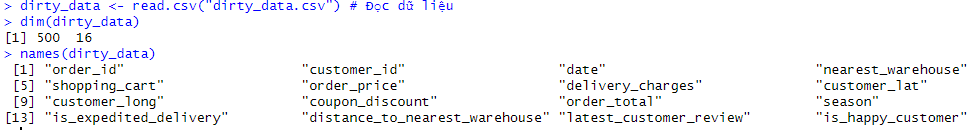
\includegraphics[width=\textwidth]{graphics/Pre_processing_data/f1.PNG}
    \caption{Kết quả của hàm dim() và names()}
    \label{f1}
\end{figure}

\subsection{Làm sạch dữ liệu}
Sau khi xem qua dữ liệu, nhóm nhận thấy dữ liệu có những lỗi sau: các giá trị trong biến \textbf{date}, \textbf{season}, \textbf{nearest\_warehouse} chưa thống nhất về định dạng; có sự sai lệch giữa một số giá trị của biến \textbf{order\_total} và giá trị tổng giá tiền được tính từ các bién \textbf{order\_price}, \textbf{delivery\_charges}, \textbf{coupon\_dis-\\
count}; có một số giá trị của biến \textbf{nearest\_warehouse} được xác định sai từ tọa độ của khách hàng và 3 nhà kho.

\subsubsection{Điều chỉnh định dạng của biến date}
Chúng ta sẽ thực hiện việc chuẩn hóa và chuyển đổi biến \textbf{date} thành định dạng ``Date'' từ dữ liệu ban đầu để đảm bảo tính nhất quán trong phân tích. Thư viện \textbf{lubridate} sẽ được sử dụng vì nó cung cấp cho ta hàm \textbf{parse\_date\_time()} giúp phân tích và chuyển đổi các giá trị trong \textbf{dirty\_data\$date} về dạng thống nhất, dựa trên các mẫu định dạng được chỉ định trong \textbf{orders = c(``ymd", ``dmy", ``mdy")}. Sau đó, sử dụng hàm \textbf{as.Date()} để đưa giá trị về định dạng ``Date''. Kết quả cho 10 giá trị đầu tiên có được biểu diễn trong hình \ref{f2}
\begin{figure}[!htbp]
    \centering
    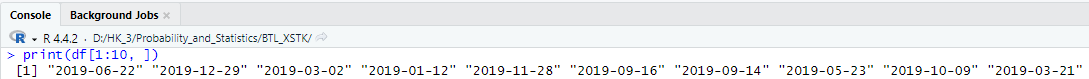
\includegraphics[width=\textwidth]{graphics/Pre_processing_data/f2.PNG}
    \caption{10 giá trị đầu tiên của biến \textbf{date} sau khi được sửa}
    \label{f2}
\end{figure} 
\subsubsection{Điều chỉnh định dạng biến season}
Ta sẽ tiến hành chỉnh sửa lại biến \textbf{season} dựa trên biến \textbf{date}. Biến \textbf{sum} được khởi tạo và được gán giá trị của <ngày trong tháng> + <tháng>\times100. Như vậy, tùy vào giá trị của \textbf{sum} mà ta sẽ xác định mùa tương ứng: Nếu \textbf{sum} nằm trong khoảng từ 301 (1 tháng 3) đến 530 (30 tháng 5), mùa được gán là Autumn (mùa thu); nếu \textbf{sum} nằm trong khoảng từ 601 (1 tháng 6) đến 831 (31 tháng 8), mùa là Winter (mùa đông); nếu \textbf{sum} nằm trong khoảng từ 901 (1 tháng 9) đến 1130 (30 tháng 11), mùa là Spring (mùa xuân); các giá trị còn lại (như từ 1 tháng 1 đến 28/29 tháng 2, hoặc tháng 12) được gán là Summer (mùa hè). (Ví dụ: Nếu ngày là 15/03, thì sum = 15 + 3 \times 100 = 315 và \textbf{season} được gán giá trị Autumn). Hình \ref{f3} thể hiện 10 giá trị của \textbf{season} trước và sau khi được sửa.
\begin{figure}[!htbp]
    \centering
    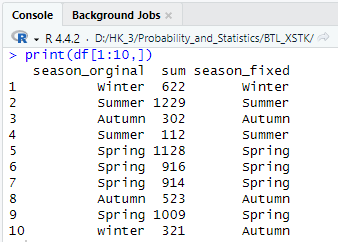
\includegraphics[width=0.3\textwidth]{graphics/Pre_processing_data/f3.PNG}
    \caption{Biến \textbf{season} trước và sau khi được tinh chỉnh}
    \label{f3}
\end{figure}

\subsubsection{Điều chỉnh tên kho hàng trong biến nearest\_warehouse}

Ta tiến hành việc chuẩn hóa dữ liệu trong bi nearest\_warehouse của tập dữ liệu dirty\_data bằng cách chuyển đổi tất cả các tên (``Thompson'', ``Nickolson'',  ``Bakers'') thành dạng Title Case (chữ cái đầu viết hoa). Thư viện \textbf{stringr} cung cấp hàm \textbf{str\_to\_title} dùng để chuyển đổi chuỗi ký tự sang dạng Title Case. Mục đích của việc chuẩn hóa định dạng văn bản này là để tăng tính nhất quán trong dữ liệu và cải thiện tính dễ đọc khi hiển thị hoặc sử dụng trong các báo cáo, phân tích. Hình \ref{f4} cho thấy hàm \textbf{unique()} được dùng để kiểm chứng việc định dạng lại dữ liệu.
\begin{figure}[!htbp]
    \centering
    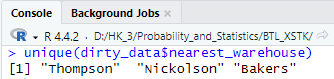
\includegraphics[width=0.3\textwidth]{graphics/Pre_processing_data/f4.PNG}
    \caption{Sử dụng hàm \textbf{unique()} để kiểm chứng kết quả}
    \label{f4}
\end{figure}

\subsubsection{Điều chỉnh giá trị trong biến order\_total}
Ta sẽ tiến hành thực hiện các bước để tính toán lại tổng chi phí (\textbf{order\_total}) của các đơn hàng dựa trên các yếu tố liên quan (\textbf{order\_price}, \textbf{delivery\_charges}, \textbf{coupon\_discount}) và kiểm tra xem có sự khác biệt nào so với dữ liệu gốc hay không. Tổng chi phí đơn hàng được tính theo công thức \textbf{calculated\_order\_total} = \textbf{order\_price} \times (1 - \textbf{coupon\_discount}/100) + \textbf{delivery\_charges}. Công thức này áp dụng giảm giá (dựa trên phần trăm \textbf{coupon\_discount}) và cộng phí giao hàng (\textbf{delivery\_charges}) để tính tổng chi phí thực tế. Việc tính lại tổng chi phí đơn hàng là để kiểm tra tính đúng đắn của dữ liệu gốc, đồng thời phát hiện và sửa lỗi (nếu có) trong dữ liệu \textbf{order\_total}. Hình \ref{f5} biểu diễn một vài giá trị ban đầu của dữ liệu bị sai và được tính toán lại thành giá trị chính xác hơn.
\begin{figure}[!htbp]
    \centering
    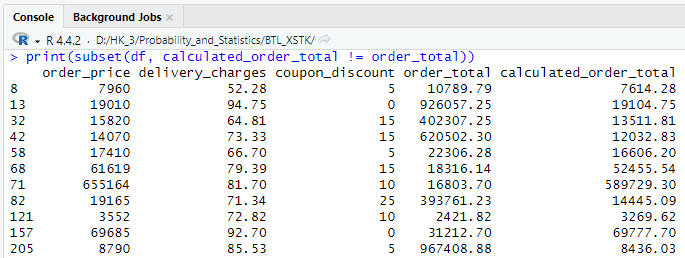
\includegraphics[width=0.7\textwidth]{graphics/Pre_processing_data/f5.PNG}
    \caption{Giá trị gốc bị lỗi của \textbf{order\_total}} được cập nhật bởi giá trị mới từ \textbf{calculated\_order\_total} 
    \label{f5}
\end{figure}

\subsubsection{Điều chỉnh giá trị trong biến nearest\_warehouse}
Ta sẽ sử dụng công thức Haversine (được trình bày trong phần \ref{Kien thuc nen}) để tính khoảng cách giữa hai điểm dựa trên tọa độ vĩ độ và kinh độ, sử dụng bán kính Trái Đất là 6371 km. Công thức được áp dụng để đo khoảng cách theo đường cong bề mặt Trái Đất, phù hợp cho dữ liệu địa lý. Hàm \textbf{haversine\_distance()} được nhóm thiết kế để tính khoảng cách từ khách hàng đến mỗi kho hàng, với đầu vào là tọa độ khách hàng và tọa độ nhà kho, hàm trả về khoảng cách giữa hai tọa độ trên. Sau khi hoàn tất việc tính khoảng cách từ một khách hàng bất kỳ đến cả 3 kho hàng, hàm \textbf{pmin()} được dùng để chọn ra kho hàng gần nhất và gán vào \textbf{distance\_to\_nearest\_warehouse\_fixed}. Hình \ref{f6} cho thấy một vài giá trị khoảng cách được tính lại có độ sai lệch bất thường so với giá trị gốc. Sau khi tìm hiểu nguyên nhân, nhóm đã phát hiện giá trị \textbf{customer\_lat} tương ứng với những khoảng cách này xấp xỉ 37 trong khi hầu hết các giá trị cùng loại khác xấp xỉ -37. Điều này dẫn nhóm đến kết luận có sự sai sót (thiếu dấu âm) trong khâu nhập dữ liệu. Cuối cùng nhóm quyết định sẽ thêm dấu âm cho các giá trị lỗi đã đề cập. Hình \ref{f7} liệt kê tất cả các giá trị của \textbf{nearest\_warehouse} bị lỗi được cập nhật lại, số lượng các giá trị lỗi này được giảm đáng kể, chứng tỏ kết luận trên là đúng đắn.
\begin{figure}[!htbp]
    \centering
    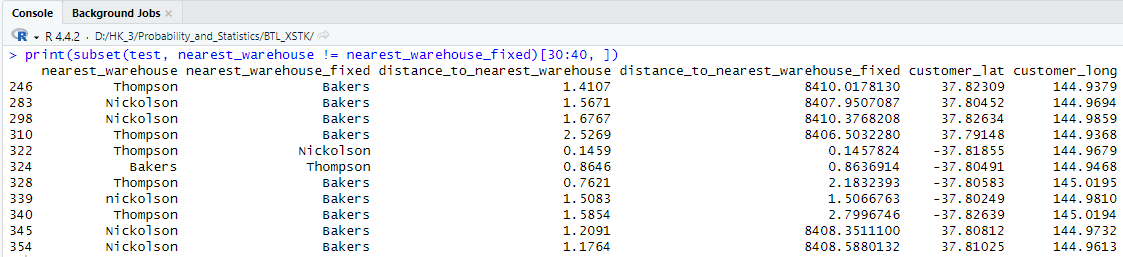
\includegraphics[width=\textwidth]{graphics/Pre_processing_data/f6.PNG}
    \caption{Một vài giá trị khoảng cách gốc và giá trị khoảng cách được tính lại}
    \label{f6}
\end{figure}
\begin{figure}[!htbp]
    \centering
    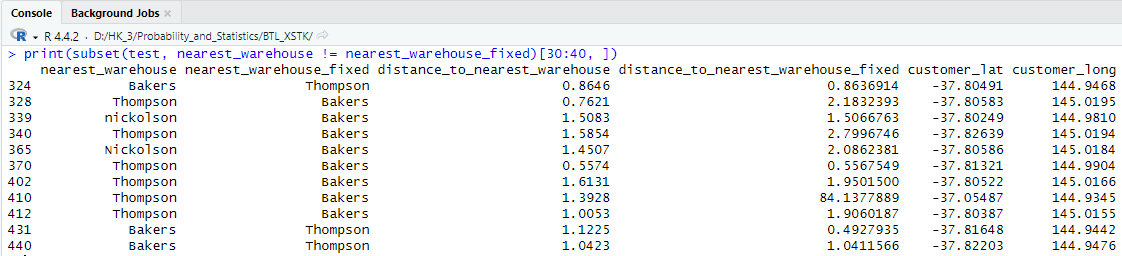
\includegraphics[width=\textwidth]{graphics/Pre_processing_data/f7.PNG}
    \caption{Các giá trị \textbf{nearest\_warehouse} lỗi được cập nhật}
    \label{f7}
\end{figure}